% Options for packages loaded elsewhere
% Options for packages loaded elsewhere
\PassOptionsToPackage{unicode}{hyperref}
\PassOptionsToPackage{hyphens}{url}
\PassOptionsToPackage{dvipsnames,svgnames,x11names}{xcolor}
%
\documentclass[
  letterpaper,
  DIV=11,
  numbers=noendperiod]{scrartcl}
\usepackage{xcolor}
\usepackage{amsmath,amssymb}
\setcounter{secnumdepth}{5}
\usepackage{iftex}
\ifPDFTeX
  \usepackage[T1]{fontenc}
  \usepackage[utf8]{inputenc}
  \usepackage{textcomp} % provide euro and other symbols
\else % if luatex or xetex
  \usepackage{unicode-math} % this also loads fontspec
  \defaultfontfeatures{Scale=MatchLowercase}
  \defaultfontfeatures[\rmfamily]{Ligatures=TeX,Scale=1}
\fi
\usepackage{lmodern}
\ifPDFTeX\else
  % xetex/luatex font selection
\fi
% Use upquote if available, for straight quotes in verbatim environments
\IfFileExists{upquote.sty}{\usepackage{upquote}}{}
\IfFileExists{microtype.sty}{% use microtype if available
  \usepackage[]{microtype}
  \UseMicrotypeSet[protrusion]{basicmath} % disable protrusion for tt fonts
}{}
\makeatletter
\@ifundefined{KOMAClassName}{% if non-KOMA class
  \IfFileExists{parskip.sty}{%
    \usepackage{parskip}
  }{% else
    \setlength{\parindent}{0pt}
    \setlength{\parskip}{6pt plus 2pt minus 1pt}}
}{% if KOMA class
  \KOMAoptions{parskip=half}}
\makeatother
% Make \paragraph and \subparagraph free-standing
\makeatletter
\ifx\paragraph\undefined\else
  \let\oldparagraph\paragraph
  \renewcommand{\paragraph}{
    \@ifstar
      \xxxParagraphStar
      \xxxParagraphNoStar
  }
  \newcommand{\xxxParagraphStar}[1]{\oldparagraph*{#1}\mbox{}}
  \newcommand{\xxxParagraphNoStar}[1]{\oldparagraph{#1}\mbox{}}
\fi
\ifx\subparagraph\undefined\else
  \let\oldsubparagraph\subparagraph
  \renewcommand{\subparagraph}{
    \@ifstar
      \xxxSubParagraphStar
      \xxxSubParagraphNoStar
  }
  \newcommand{\xxxSubParagraphStar}[1]{\oldsubparagraph*{#1}\mbox{}}
  \newcommand{\xxxSubParagraphNoStar}[1]{\oldsubparagraph{#1}\mbox{}}
\fi
\makeatother


\usepackage{longtable,booktabs,array}
\newcounter{none} % for unnumbered tables
\usepackage{calc} % for calculating minipage widths
% Correct order of tables after \paragraph or \subparagraph
\usepackage{etoolbox}
\makeatletter
\patchcmd\longtable{\par}{\if@noskipsec\mbox{}\fi\par}{}{}
\makeatother
% Allow footnotes in longtable head/foot
\IfFileExists{footnotehyper.sty}{\usepackage{footnotehyper}}{\usepackage{footnote}}
\makesavenoteenv{longtable}
\usepackage{graphicx}
\makeatletter
\newsavebox\pandoc@box
\newcommand*\pandocbounded[1]{% scales image to fit in text height/width
  \sbox\pandoc@box{#1}%
  \Gscale@div\@tempa{\textheight}{\dimexpr\ht\pandoc@box+\dp\pandoc@box\relax}%
  \Gscale@div\@tempb{\linewidth}{\wd\pandoc@box}%
  \ifdim\@tempb\p@<\@tempa\p@\let\@tempa\@tempb\fi% select the smaller of both
  \ifdim\@tempa\p@<\p@\scalebox{\@tempa}{\usebox\pandoc@box}%
  \else\usebox{\pandoc@box}%
  \fi%
}
% Set default figure placement to htbp
\def\fps@figure{htbp}
\makeatother


% definitions for citeproc citations
\NewDocumentCommand\citeproctext{}{}
\NewDocumentCommand\citeproc{mm}{%
  \begingroup\def\citeproctext{#2}\cite{#1}\endgroup}
\makeatletter
 % allow citations to break across lines
 \let\@cite@ofmt\@firstofone
 % avoid brackets around text for \cite:
 \def\@biblabel#1{}
 \def\@cite#1#2{{#1\if@tempswa , #2\fi}}
\makeatother
\newlength{\cslhangindent}
\setlength{\cslhangindent}{1.5em}
\newlength{\csllabelwidth}
\setlength{\csllabelwidth}{3em}
\newenvironment{CSLReferences}[2] % #1 hanging-indent, #2 entry-spacing
 {\begin{list}{}{%
  \setlength{\itemindent}{0pt}
  \setlength{\leftmargin}{0pt}
  \setlength{\parsep}{0pt}
  % turn on hanging indent if param 1 is 1
  \ifodd #1
   \setlength{\leftmargin}{\cslhangindent}
   \setlength{\itemindent}{-1\cslhangindent}
  \fi
  % set entry spacing
  \setlength{\itemsep}{#2\baselineskip}}}
 {\end{list}}
\usepackage{calc}
\newcommand{\CSLBlock}[1]{\hfill\break\parbox[t]{\linewidth}{\strut\ignorespaces#1\strut}}
\newcommand{\CSLLeftMargin}[1]{\parbox[t]{\csllabelwidth}{\strut#1\strut}}
\newcommand{\CSLRightInline}[1]{\parbox[t]{\linewidth - \csllabelwidth}{\strut#1\strut}}
\newcommand{\CSLIndent}[1]{\hspace{\cslhangindent}#1}



\setlength{\emergencystretch}{3em} % prevent overfull lines

\providecommand{\tightlist}{%
  \setlength{\itemsep}{0pt}\setlength{\parskip}{0pt}}



 


\KOMAoption{captions}{tableheading}
\makeatletter
\@ifpackageloaded{caption}{}{\usepackage{caption}}
\AtBeginDocument{%
\ifdefined\contentsname
  \renewcommand*\contentsname{Table of contents}
\else
  \newcommand\contentsname{Table of contents}
\fi
\ifdefined\listfigurename
  \renewcommand*\listfigurename{List of Figures}
\else
  \newcommand\listfigurename{List of Figures}
\fi
\ifdefined\listtablename
  \renewcommand*\listtablename{List of Tables}
\else
  \newcommand\listtablename{List of Tables}
\fi
\ifdefined\figurename
  \renewcommand*\figurename{Figure}
\else
  \newcommand\figurename{Figure}
\fi
\ifdefined\tablename
  \renewcommand*\tablename{Table}
\else
  \newcommand\tablename{Table}
\fi
}
\@ifpackageloaded{float}{}{\usepackage{float}}
\floatstyle{ruled}
\@ifundefined{c@chapter}{\newfloat{codelisting}{h}{lop}}{\newfloat{codelisting}{h}{lop}[chapter]}
\floatname{codelisting}{Listing}
\newcommand*\listoflistings{\listof{codelisting}{List of Listings}}
\makeatother
\makeatletter
\makeatother
\makeatletter
\@ifpackageloaded{caption}{}{\usepackage{caption}}
\@ifpackageloaded{subcaption}{}{\usepackage{subcaption}}
\makeatother
\usepackage{bookmark}
\IfFileExists{xurl.sty}{\usepackage{xurl}}{} % add URL line breaks if available
\urlstyle{same}
% fallback for those not using the hyperref driver hyperxmp:
\makeatletter
\@ifundefined{xmpquote}{\newcommand{\xmpquote}[1]{#1}}{}
\makeatother
\hypersetup{
  pdftitle={Visualizing Educational Attainment as a Lever for Upward Mobility in the District of Columbia},
  pdfauthor={Úna Gogstetter; Ayla Hauser; Simran Jayasinghe; Alice MacGarvie Thompson},
  pdfkeywords={\xmpquote{Washington, D.C}, \xmpquote{Upward
Mobility}, \xmpquote{Educational Attainment}, \xmpquote{Data
Dashboard}},
  colorlinks=true,
  linkcolor={blue},
  filecolor={Maroon},
  citecolor={Blue},
  urlcolor={Blue},
  pdfcreator={LaTeX via pandoc}}


\title{Visualizing Educational Attainment as a Lever for Upward Mobility
in the District of Columbia}
\author{Úna Gogstetter \and Ayla Hauser \and Simran
Jayasinghe \and Alice MacGarvie Thompson}
\date{2026-11-25}
\begin{document}
\maketitle
\begin{abstract}
The drastic economic disparities in Washington, District of Columbia,
often obscure the impacts of poverty and inequity upon residents living
in working-class and low-income communities. The immense wealth in parts
of the city skews citywide data and masks these impacts. This limits the
capability of city officials to use data to inform education policy.
Many data-driven projects do not examine data with such granularity as
the school, census tract, block, or neighborhood level. Projects such as
the Urban Institute's Upward Mobility Dashboard help policymakers
understand conditions affecting upward mobility. However, many of these
projects only cover data at the county level, not the census tract
level. Our project seeks to visualize and model the impacts of key
educational conditions and levers on upward mobility and educational
attainment outcomes. We use data pulled from the school, block, tract,
neighborhood, and ward levels to model this for the Department of the
Deputy Mayor for Education for the District of Columbia.
\end{abstract}


\section{Introduction}\label{introduction}

In the District of Columbia, significant disparities in resources and
economic mobility outcomes create different realities of opportunity for
residents across the district. Aggregate citywide statistics often mask
contrasts between local metrics, losing track of inequities through
broad averages of the data, an oversimplification that can be observed
when exploring poverty and income across the district.

D.C. exhibits one of the highest levels of income inequality in the
United States, where household income in the highest quintile exceeds
that of the lowest quintile by nearly 29 times (Santillo et al. 2022).
D.C.'s Gini coefficient --- which is a value between 0 and 1 where 1
signifies the greatest income inequality --- is 0.51 (U.S. Census Bureau
2023). The county encompassing the District of Columbia is above the
95th percentile for income inequality (as measured by the Gini
coefficient) among all counties in the United States (U.S. Census Bureau
2023). These economic gaps are heavily spatialized across the city's
eight wards; for instance, poverty concentrations predominantly cluster
east of the Anacostia River in Wards 7 and 8 (Naveed 2017). Since
commonly reported citywide metrics average out these regional divides,
effective policy design requires granular spatial analysis to reveal how
opportunity drivers and community resources are distributed across
specific neighborhoods.

Because educational access and environment serve as catalysts for upward
economic mobility, these systemic resource disparities directly impact
outcomes across D.C.'s public education system. To address these
structural inequities, the Office of the District of Columbia Deputy
Mayor for Education (DME) works to create conditions that support
academic acceleration across the PreK--12 public education system. The
Office of the District of Columbia Deputy Mayor for Education (DME)
works to create conditions that support educational attainment and
academic acceleration at the PreK-12 levels, focusing on schools and
their surrounding neighborhoods as sites for social and economic
justice. This work relies on granular place-based insights to inform
targeted policymaking, funding initiatives, and community programming,
and ensure these programs are guided to areas of need.

\subsection{Relevant work}\label{relevant-work}

National data visualization platforms such as the Urban Institute's
Upward Mobility Data Dashboard provide helpful insights into key
predictors of mobility indicators, but lack the neighborhood resolution
required for D.C.'s urban landscape. Without multi-scalar analytical
tools that synthesize local education and socio-economic outcomes
simultaneously, government agencies face challenges in identifying where
and how targeted interventions can close persistent opportunity gaps.

\subsection{Our contribution}\label{our-contribution}

To bridge this gap, this capstone project collaborates with the DME to
adapt and refine the Urban Institute's Upward Mobility Dashboard at the
local level. This project specifically explores the impact of
educational factors on upward mobility across the District of Columbia
by aggregating disparate indicators into a unified structure across
census tract, neighborhood, ward, and citywide scales. The project aims
to create a public-facing web application that illustrates variations in
opportunity and offers statistical analysis tools that can be used to
evaluate how targeted policy interventions can close gaps in
opportunity, providing a localized platform for public reporting,
equitable resource allocation, and data-driven decision-making.

\section{Data}\label{sec-data}

\subsubsection{Data Sources}\label{data-sources}

As we are working to create a comprehensive list of variables that
define educational attainment and upward mobility, we have been pulling
data from many different sources. For more generalized data from
Washington, D.C., we used the 2020 decennial census data, which holds
the most recent census information. We have pulled census data for every
defined census tract in Washington, D.C., which is a complete count of
every resident. It must be noted that decennial census data has the
lowest margin of error, as it is a complete count of the Washington,
D.C. population, but it can still have discrepancies in census
boundaries between years. For more up-to-date information, we have also
been accumulating data from the American Community Survey (ACS) in 2024
to observe more accurate indicators of modern D.C. environments. The ACS
allows us to collect more recent information, but it represents only a
small subset of the D.C. population, as it is an annual survey that is
optionally completed.

Additionally, our sponsors shared data from both EdScape and Open Data
DC and identified variables that seemed the most important for the goals
of the project. Open Data DC is managed by the Enterprise Data team in
the Office of the Chief Technology Officer and uses city government open
data (Office of the Chief Technology Officer 2026). ED Scape, created by
the Office of the Deputy Mayor of Education (DME), carries downloadable
data sets from the DME specific to schools in Washington, DC (Office of
the Deputy Mayor for Education 2026). Cumulatively, the data is counted
by populations, percentages, counts, and estimates in a specific D.C.
ward, block, tract, or neighborhood. Most of our data can be pulled
remotely; for functionality, we have our data pulled at the user's
choice, not constantly.

\subsubsection{Data Description}\label{data-description}

We have categorized all of the outcome data and their corresponding
variables into different categories for upward mobility in
Table~\ref{tbl-outcome-categories} below. These can be broken down into
5 main categories: economic opportunity \& housing affordability,
demographic diversity, public safety \& neighborhood quality,
transportation \& recreational access, and built environment indicators.
Economic Opportunity \& Housing Affordability covers poverty, income,
rent, and affordable housing variables. Demographic diversity explores
the percent of different ethnicity and nationalities. Public Safety \&
Neighborhood Quality highlights land use, crime, and parks \&
recreation. Transit \& Recreational Access includes variables such as
child development centers and transit stops per capital. The built
environment indicators are divided into the subcategories: access to
school, parks \& recreation access, safety and wellness indicators,
access to transit, public safety \& tract infrastructure, digital access
\& educational resources, economic \& financial access, food access, and
climate resilience. Ultimately, our outcome data compiles into 53
different observable variables and 14,393 observations. Most of our data
can be visualized across neighborhood, ward, and census tract. However,
total population, percentage race, percentage renter-occupied, and
percent owner-occupied data are only available by D.C. block level.

\begin{longtable}[]{@{}
  >{\raggedright\arraybackslash}p{(\linewidth - 8\tabcolsep) * \real{0.2308}}
  >{\raggedright\arraybackslash}p{(\linewidth - 8\tabcolsep) * \real{0.1897}}
  >{\raggedright\arraybackslash}p{(\linewidth - 8\tabcolsep) * \real{0.1385}}
  >{\raggedright\arraybackslash}p{(\linewidth - 8\tabcolsep) * \real{0.1385}}
  >{\raggedright\arraybackslash}p{(\linewidth - 8\tabcolsep) * \real{0.3026}}@{}}

\caption{\label{tbl-outcome-categories}Categorized Outcome Variables}

\tabularnewline

\toprule\noalign{}
\begin{minipage}[b]{\linewidth}\raggedright
Category
\end{minipage} & \begin{minipage}[b]{\linewidth}\raggedright
Variable 1
\end{minipage} & \begin{minipage}[b]{\linewidth}\raggedright
Variable 2
\end{minipage} & \begin{minipage}[b]{\linewidth}\raggedright
Variable 3
\end{minipage} & \begin{minipage}[b]{\linewidth}\raggedright
Variable 4
\end{minipage} \\
\midrule\noalign{}
\endhead
\bottomrule\noalign{}
\endlastfoot
Economic Opportunity \& Housing Affordability & Poverty Rate & Median
Household Income & Median Rent & Affordable Housing Units Constructed
Since 2015 Per Capita \\
Demographic Diversity & Percent Foreign-born & Percent White Only & NA &
NA \\
Public Safety \& Neighborhood Quality & Land Use Diversity Score (0-1) &
Percent Positive Land Uses & Parks Per Capita & Crimes Per Capita \\
Transportation \& Recreational Access & Child Development Centers Per
Capita & Transit Stops Per Capita & NA & NA \\
Built Environment Indicators & Access to School & Parks + Recreation
Access & Safety Wellness Indicators & Access to Transit \\

\end{longtable}

\textsubscript{Source:
\href{https://sds-capstone.github.io/dced-f26/index.qmd.html}{Article
Notebook}}

Our predictor variables have 4 main categories: attendance, graduation
\& college enrollment, enrollment, level of educational attainment, and
employment, with some available by DC school district and others by
census tract (Table~\ref{tbl-predictor-categories})

\begin{longtable}[]{@{}
  >{\raggedright\arraybackslash}p{(\linewidth - 8\tabcolsep) * \real{0.2485}}
  >{\raggedright\arraybackslash}p{(\linewidth - 8\tabcolsep) * \real{0.1576}}
  >{\raggedright\arraybackslash}p{(\linewidth - 8\tabcolsep) * \real{0.1879}}
  >{\raggedright\arraybackslash}p{(\linewidth - 8\tabcolsep) * \real{0.2000}}
  >{\raggedright\arraybackslash}p{(\linewidth - 8\tabcolsep) * \real{0.2061}}@{}}

\caption{\label{tbl-predictor-categories}Categorized Predictor
Variables}

\tabularnewline

\toprule\noalign{}
\begin{minipage}[b]{\linewidth}\raggedright
Category
\end{minipage} & \begin{minipage}[b]{\linewidth}\raggedright
Variable 1
\end{minipage} & \begin{minipage}[b]{\linewidth}\raggedright
Variable 2
\end{minipage} & \begin{minipage}[b]{\linewidth}\raggedright
Variable 3
\end{minipage} & \begin{minipage}[b]{\linewidth}\raggedright
Variable 4
\end{minipage} \\
\midrule\noalign{}
\endhead
\bottomrule\noalign{}
\endlastfoot
Attendance (OSSE) & Chronic Absenteeism Rate & Pre-K Chronic Absenteeism
Rate & Attendance Growth & NA \\
Graduation and College Enrollment (OSSE) & Four-Year Graduation Rate &
Five-Year Graduation Rate & 6-Month Postsecondary Enrollment & 12-Month
Postsecondary Enrollment \\
Enrollment (ACS) & Nursery school, preschool & Kindergarten Enrollment &
NA & NA \\
Level of Educational Attainment (ACS) & High School Graduate &
Bachelor's or higher & NA & NA \\
Employment(ACS) & Employment Rate Age 20-24 & Employment Rate Age 25-29
& NA & NA \\

\end{longtable}

\textsubscript{Source:
\href{https://sds-capstone.github.io/dced-f26/index.qmd.html}{Article
Notebook}}

\subsubsection{Data Cleaning and
Preparation}\label{data-cleaning-and-preparation}

All data sets were imported and cleaned individually to best suit the
type of visualizations our sponsor wanted to observe. Each individual
data set was eventually comprised of 6 columns: \texttt{variable},
\texttt{estimate}, \texttt{short\_name}, \texttt{neighborhood},
\texttt{ward}, and \texttt{geometry}. \texttt{Variable} corresponds to
the specific variable the data is examining (i.e., ``Poverty Rate'',
``Median Household Income''). \texttt{Estimate} is the given measure of
the data and can be represented as a count or a percentage.
\texttt{short\_name} corresponds to the census tract that each estimate
is a total for. The last three columns contain the specific
neighborhood, ward, and polygon geometry for which each estimate is a
count. Each of the 53 variables was weighted across the census,
neighborhood, and ward populations. We included NA values, but converted
them to a string called ``No Data'' for better readability in the
visualizations.

\subsubsection{Summary Statistics and Exploratory Data
Analysis}\label{summary-statistics-and-exploratory-data-analysis}

Overall, our combined data contains 14,393 rows (observations), 53
variables, 206 tracts, 107 neighborhoods, and 8 wards. To contextualize
the spatial demographics of the number of census tracts to
neighborhoods, we have provided Figure~\ref{fig-tracts} below.

\protect\phantomsection\label{cell-fig-tracts}
\begin{figure}[H]

\centering{

\pandocbounded{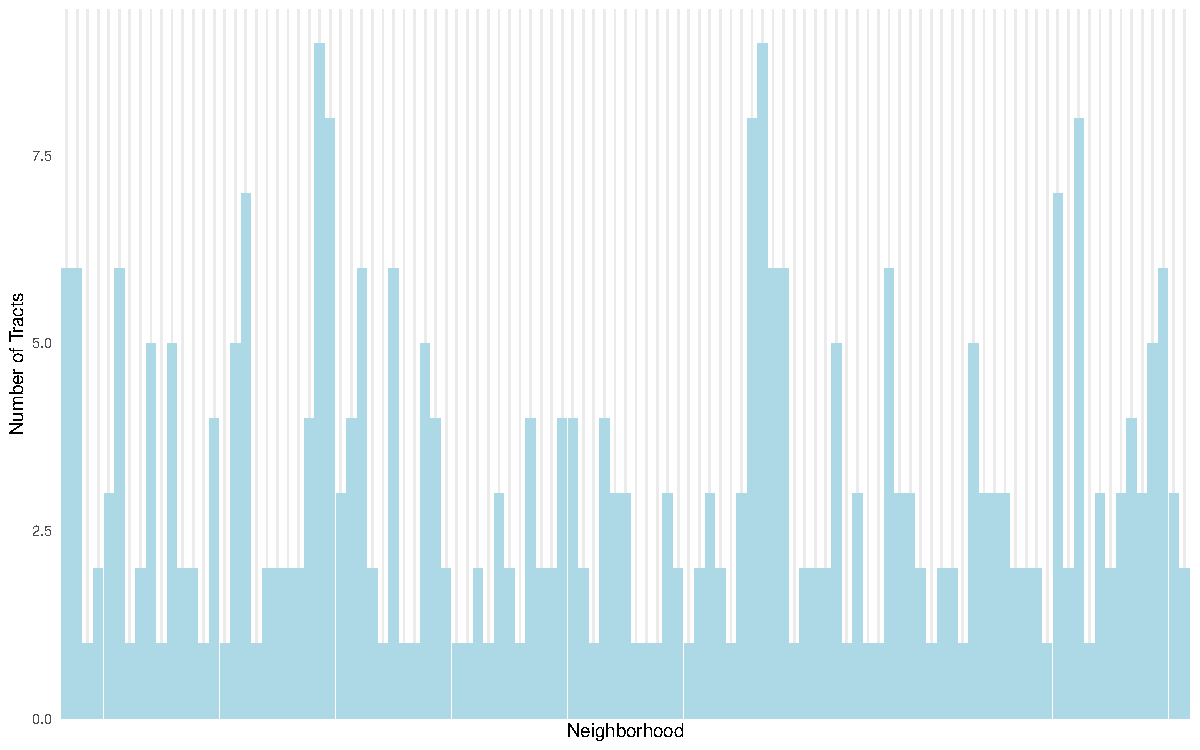
\includegraphics[keepaspectratio]{index_files/figure-pdf/fig-tracts-1.pdf}}

}

\caption{\label{fig-tracts}Number of Census Tracts per D.C.
Neighborhood}

\end{figure}%

\textsubscript{Source:
\href{https://sds-capstone.github.io/dced-f26/index.qmd.html}{Article
Notebook}}

Most neighborhoods are made up of 1-2 census tracts, but some has as
many as 8-9 census tracts, thus we must weight for population in our
analyses.

For simplicity, the rest of this exploratory data analysis will contain
6 key variables that represent each of our outcome categories: poverty,
percent foreign-born, parks per capita, child development centers per
capita, percent tract within a 15-minute walk of a health care facility,
and the predictor variable: chronic absenteeism rate.

\begin{longtable}[]{@{}
  >{\raggedright\arraybackslash}p{(\linewidth - 10\tabcolsep) * \real{0.5310}}
  >{\raggedleft\arraybackslash}p{(\linewidth - 10\tabcolsep) * \real{0.0973}}
  >{\raggedleft\arraybackslash}p{(\linewidth - 10\tabcolsep) * \real{0.0619}}
  >{\raggedleft\arraybackslash}p{(\linewidth - 10\tabcolsep) * \real{0.1681}}
  >{\raggedleft\arraybackslash}p{(\linewidth - 10\tabcolsep) * \real{0.0708}}
  >{\raggedleft\arraybackslash}p{(\linewidth - 10\tabcolsep) * \real{0.0708}}@{}}

\caption{\label{tbl-summary-stats}Summary Statistics for Key Variables}

\tabularnewline

\toprule\noalign{}
\begin{minipage}[b]{\linewidth}\raggedright
Variable
\end{minipage} & \begin{minipage}[b]{\linewidth}\raggedleft
Mean
\end{minipage} & \begin{minipage}[b]{\linewidth}\raggedleft
Median
\end{minipage} & \begin{minipage}[b]{\linewidth}\raggedleft
Standard Deviation
\end{minipage} & \begin{minipage}[b]{\linewidth}\raggedleft
Minimum
\end{minipage} & \begin{minipage}[b]{\linewidth}\raggedleft
Maximum
\end{minipage} \\
\midrule\noalign{}
\endhead
\bottomrule\noalign{}
\endlastfoot
\% of Students Chronically Absent, 24-25 & 38.2189655 & 38.850 &
20.4043811 & 6.40 & 98.40 \\
Percent Foreign-Born & 14.0771845 & 12.450 & 9.2802604 & 0.00 & 48.20 \\
Percent Positive Land Uses & 85.4900971 & 88.765 & 13.0309441 & 45.33 &
100.00 \\
Percent Tract Within 15-Minute Walk of Health Care Facility & 88.6195631
& 99.990 & 24.4194560 & 0.00 & 99.99 \\
Poverty Rate (\%) & 16.3519417 & 11.100 & 14.8172336 & 0.00 & 100.00 \\
Transit Stops Per Capita & 0.0090291 & 0.000 & 0.0678451 & 0.00 &
0.97 \\

\end{longtable}

\textsubscript{Source:
\href{https://sds-capstone.github.io/dced-f26/index.qmd.html}{Article
Notebook}}

In Table~\ref{tbl-summary-stats}, there is a quick summary of the
statistics between our key variables. We can see that there is high
variation in most of the data with standard deviations in the 10s and
20s. Additionally, a lot of our percentages have minimums of 0\% and
maximums of 100\%, highlighting the variety within the D.C. tract
environments. To better observe data variation across D.C.,
Figure~\ref{fig-ward} displays the variation of estimates across the key
variables for each ward.

\protect\phantomsection\label{cell-fig-ward}
\begin{figure}[H]

\centering{

\pandocbounded{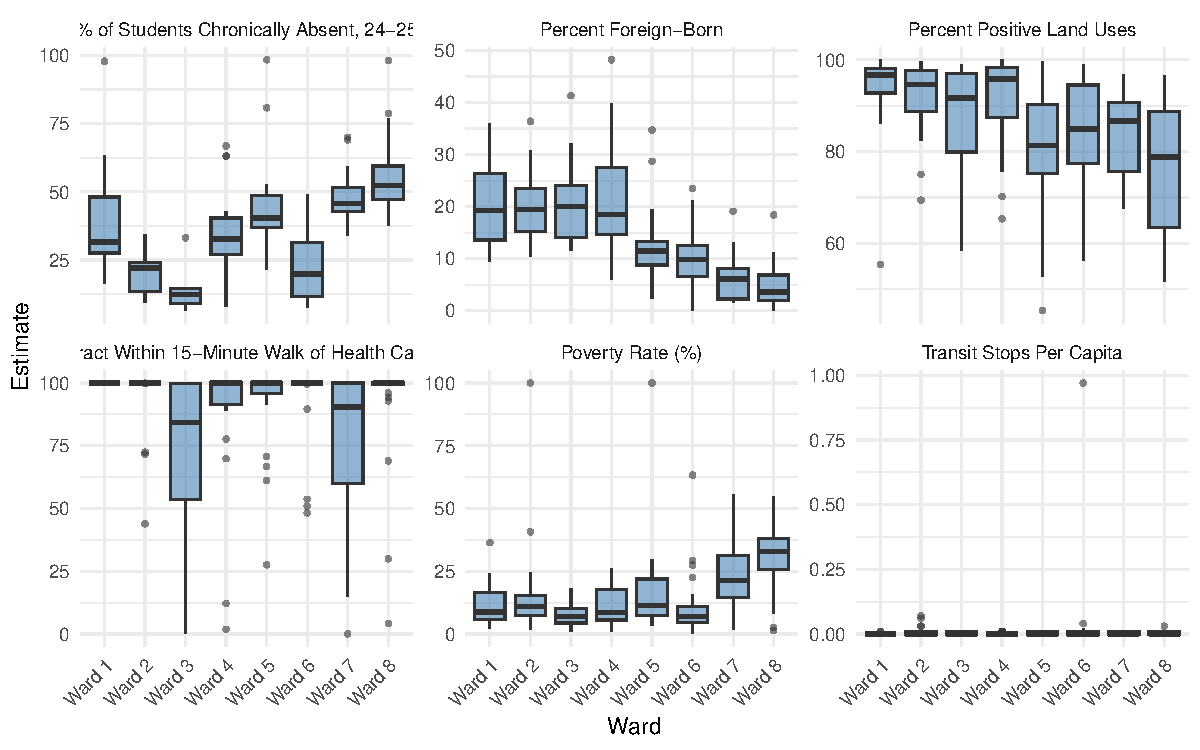
\includegraphics[keepaspectratio]{index_files/figure-pdf/fig-ward-1.pdf}}

}

\caption{\label{fig-ward}Key Variables estimates by Ward}

\end{figure}%

\textsubscript{Source:
\href{https://sds-capstone.github.io/dced-f26/index.qmd.html}{Article
Notebook}}

As aforementioned, D.C. is characterized by its variable discrepancies
across the city. This is highlighted in Figure~\ref{fig-ward} where we
say great variation in the percent of students chronically absent,
percent positive lang uses, poverty rates, and percent foreign born. It
is to be noted that Ward 6 is unique in that this is near the capital
where few live, so there are more transit stops per capita. While
exploring variation in the city is beneficial, we are increasingly
interested in the relationship between these variables. These
relationships are exemplified in Figure~\ref{fig-cor}.

\protect\phantomsection\label{cell-fig-cor}
\begin{figure}[H]

\centering{

\pandocbounded{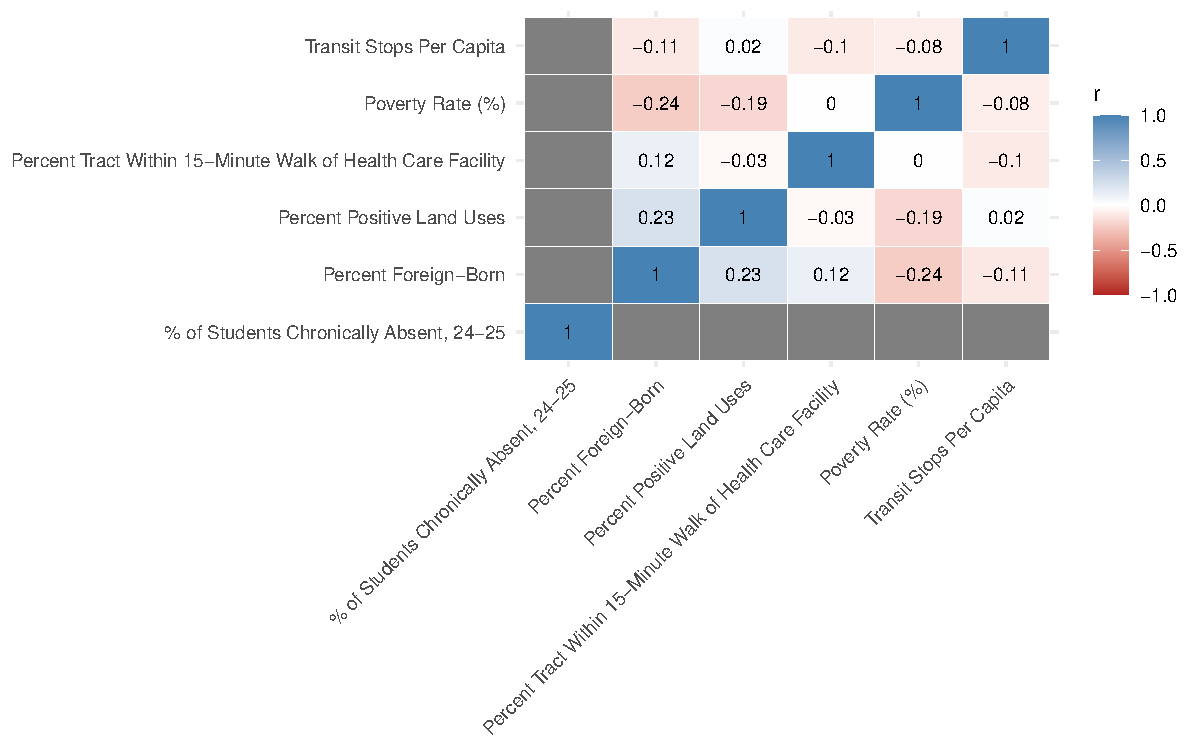
\includegraphics[keepaspectratio]{index_files/figure-pdf/fig-cor-1.pdf}}

}

\caption{\label{fig-cor}Heatmap of Correlation Coefficients for each Key
Variable}

\end{figure}%

\textsubscript{Source:
\href{https://sds-capstone.github.io/dced-f26/index.qmd.html}{Article
Notebook}}

It can be observed that there is light, negative correlation between
most variables. However, the relationship between poverty rate and
percent of students chronically absent (-0.24), highlights the
possibility of a stronger correlation. Additionally, we see few positive
correlations, with the strongest between percent positive land uses and
percent foreign born (0.23).

\section{Methods}\label{sec-methods}

\begin{quote}
Methods: What did you actually do? What techniques or methods did you
employ? What were the specifications for any statistical models you
used? What software or packages did you use or develop?
\end{quote}

\section{Results}\label{results}

\begin{quote}
Results: What did you learn about the problem you identified in Section
1? This is where you put the tables, figures, and analytics by-products
of your work.
\end{quote}

\section{Conclusion}\label{conclusion}

\begin{quote}
Conclusion: What are the limitations of your work? What are some next
steps that someone (either you or another research group) should
consider in attempting to further your work? Remind us one last time
about what you did.
\end{quote}

\subsection{Limitations}\label{limitations}

\subsection{Future work}\label{future-work}

\subsection{Final thoughts}\label{final-thoughts}

\section{Ethical statement}\label{ethical-statement}

\begin{quote}
Drawing on what you have learned about data science ethics in this
class, discuss any ethical considerations in your project. For some
projects, this statement could be quite short (one paragraph may
suffice). For other projects, more detail may be needed (no more than 2
pages).

Be expansive and creative in your thinking about \textbf{possible}
ethical considerations. One way to do this assignment poorly would be to
write a short statement asserting that there are no ethical
considerations, only to have me think of several fairly obvious ones.
\end{quote}

\section{Acknowledgements}\label{acknowledgements}

\begin{quote}
Were there any people or organizations who helped you that you would
like to acknowledge?
\end{quote}

\section*{References}\label{references}
\addcontentsline{toc}{section}{References}

\begin{quote}
References: Every reference (except for books) needs a DOI (strongly
preferred) or URL. Use \href{https://scholar.google.com}{Google Scholar}
to help with BibTeX. Every book needs publisher location (e.g.~``City,
ST: Publisher''). 🙄 See
\href{https://smithcollege-sds.github.io/sds100/lab_12_bibliographies.html}{SDS
100: Bibliographies}
\end{quote}

\protect\phantomsection\label{refs}
\begin{CSLReferences}{1}{1}
\bibitem[\citeproctext]{ref-naveed2017income}
Naveed, Minahil. 2017. {``Income Inequality in {DC} Highest in the
Country.''} DC Fiscal Policy Institute, December 15.
\url{https://dcfpi.org/all/income-inequality-dc-highest-country-2/}.

\bibitem[\citeproctext]{ref-opendatadc}
Office of the Chief Technology Officer. 2026. {``{Open Data DC}.''}
\url{https://opendata.dc.gov/}.

\bibitem[\citeproctext]{ref-edscape}
Office of the Deputy Mayor for Education. 2026. {``{EDScape}.''}
\url{https://edscape.dc.gov/}.

\bibitem[\citeproctext]{ref-santillo2022washingtondc}
Santillo, Miranda, Mingli Zhong, and Oriya Cohen. 2022. {``Washington,
{DC}, Has Glaring Financial Health Inequities. So Do Most {American}
Cities. Urban Wire.''} Urban Institute, October 6.
\url{https://www.urban.org/urban-wire/washington-dc-has-glaring-financial-health-inequities-so-do-most-american-cities}.

\bibitem[\citeproctext]{ref-Census2023ACSDT5Y2023}
U.S. Census Bureau. 2023. {``Gini Index of Income Inequality.''} U.S.
Department of Commerce.
\url{https://data.census.gov/table/ACSDT5Y2023.B19083?q=income+inequality&g=010XX00US\%240500000}.

\end{CSLReferences}




\end{document}
